%----------------------------------------------------------------------------------------
%	PACKAGES AND OTHER DOCUMENT CONFIGURATIONS
%----------------------------------------------------------------------------------------

\documentclass[fleqn,10pt]{SelfArx} % Document font size and equations flushed left

\usepackage[english]{babel}
\usepackage{lipsum}
\usepackage{graphicx}
\usepackage{algorithm}
\usepackage{algpseudocode}
\usepackage{amsmath}
\usepackage{listings}
\usepackage{xcolor}
\usepackage{minted}
\usepackage{pgfplots}
\usepackage{tabularx}

% ----------------------------------------------------------------------------------------
% 	CONFIGURATIONS
% ----------------------------------------------------------------------------------------
\pgfplotsset{compat=1.18}
\newsavebox\mysavebox

%----------------------------------------------------------------------------------------
%	COLUMNS
%----------------------------------------------------------------------------------------

\setlength{\columnsep}{0.55cm} % Distance between the two columns of text
\setlength{\fboxrule}{0.75pt} % Width of the border around the abstract

%----------------------------------------------------------------------------------------
%	COLORS
%----------------------------------------------------------------------------------------

\definecolor{color1}{RGB}{0,0,90} % Color of the article title and sections
\definecolor{color2}{RGB}{0,20,20} % Color of the boxes behind the abstract and headings

\definecolor{commentcolor}{rgb}{0.0, 0.5, 0.0}
\definecolor{keywordcolor}{rgb}{0.13, 0.13, 1.0}
\definecolor{stringcolor}{rgb}{0.58, 0.0, 0.82}

\lstset{
    keywordstyle=\color{keywordcolor}\bfseries,
    commentstyle=\color{commentcolor},
    stringstyle=\color{stringcolor},
    basicstyle=\ttfamily,
    numbers=left,
    numberstyle=\tiny\color{gray},
    frame=single,
    breaklines=true,
    showstringspaces=false
}

%----------------------------------------------------------------------------------------
%	HYPERLINKS
%----------------------------------------------------------------------------------------

\usepackage{hyperref}

\hypersetup{
	hidelinks,
	colorlinks,
	breaklinks=true,
	urlcolor=color2,
	citecolor=color1,
	linkcolor=color1,
	bookmarksopen=false,
	pdftitle={Title},
	pdfauthor={Author},
}

%----------------------------------------------------------------------------------------
%	ARTICLE INFORMATION
%----------------------------------------------------------------------------------------

\JournalInfo{ENGN3712: Major Research Project}
\Archive{Mid Project Report}

\PaperTitle{Bringing Extract Method Refactoring to the Rust Programming Language:
Experiments with REM}

\Authors{Matthew Britton\textsuperscript{1}, Supervisor: Alex Potanin\textsuperscript{2}}
\affiliation{\textsuperscript{1}\textit{School of Engineering, The Australian
National University. | matt.britton@anu.edu.au}}
\affiliation{\textsuperscript{2}\textit{School of Computing, The Australian
National University. | alex.potanin@anu.edu.au}}

\Keywords{}
\newcommand{\keywordname}{Keywords}

%----------------------------------------------------------------------------------------
%	ABSTRACT
%----------------------------------------------------------------------------------------

\Abstract{Lorem ipsum dolor sit amet, consectetur adipiscing elit. Sed auctor, nunc nec}

%----------------------------------------------------------------------------------------

\begin{document}

\maketitle

\tableofcontents


%----------------------------------------------------------------------------------------
%	ARTICLE CONTENTS
%----------------------------------------------------------------------------------------

\section{Introduction}

\section{Theory Work Completed to Date}

\subsection*{Literature Review Progress}

A literature review is in the process of being written, and is around 60-75\%
complete. A draft will be completed by the Christmas break, and it will be
finished by the end of the summer break (although it will still be subject to
review and future revisions). It (broadly) covers the following topics, with
topics marked with * potentially being added:
\begin{itemize}[itemsep=0pt]
    \item An Overview of Extract Method Refactoring.
    \item Rust's Memory Management Model (Ownership and Borrowing), and how its'
    type system both helps and hinders refactoring tools.
    \item * Evolving Standards and Best Practices in the Rust Ecosystem.
    \item Existing Refactoring Tools and Their Limitations.
    \item Previous Work on the REM Tool by Ilya Sergey et al and Sewen Thy.
    \item Advanced Refactoring Techniques in Other Languages.
    \item Testing and Validation Strategies for Refactoring Tools
    \item * Comparative Analysis with Other Programming Languages.
    \item * Integration with Developer Tools.
\end{itemize}

\subsection*{Research into Advanced Refactoring Methods}

Recent research on advanced refactoring methods, primarily focused on Java,
highlights the importance of enhancing tools to handle the complexities of
asynchronous programming and generics. Lin et al. developed ASYNCDROID \cite{AndroidAsncRefactoring}, a tool
that refactors improperly used Android async constructs, transforming them into
more efficient forms like \verb|IntentService|. This approach
addresses memory leaks and lost results, by automating these complex refactorings. \\
Similarly, Zhang et al. proposed ReFuture \cite{AutomaticRefactoringAsyncJAVA}, a tool for automating refactoring in
Java projects using CompletableFuture, improving asynchronous code efficiency
through static analysis techniques like visitor pattern and alias
analysis. This tool demonstrated high effectiveness in large
codebases, emphasizing the need for advanced analysis to manage dependencies and
optimize task scheduling. \\
Additionally, Marticorena et al. explored the impact of generics on method
extraction refactorings in Java, noting the necessity for refactoring tools to
evolve as programming languages incorporate more sophisticated type
systems \cite{GenericRefactoringJAVA}. \\
These studies, while centered on Java, underscore the broader need for
developing refactoring methods for modern language features, particularly in
environments with strict memory and type constraints.

\section{Coding Progress}

\subsection*{Modifications to REM}

The most important modification to the original toolchain has been decoupling it
from the rust compiler. Previously, REM was heavily tied to rustc, the rust
compiler. It relied compiler specific representations of files and their syntax
trees. Because of this dependency, REM required a very specific buildchain, and
could not be used outside of this build context. Additionally, when I took over
the project, changes to external libraries meant that the toolchain was
completely non-functional. Some work is still required to bring the toolchain
off of nightly rust onto stable rust.\\
Another small modification has been changing the way REM handles data.
Previously, the three main components of REM (controller, borrower and repairer)
worked by each reading and writing to a file, and then passing the file to the
next stage of the toolchain. By changing the way data is passed between the (now
5) modules of REM, a roughly 10-20\% speedup has been achieved.

\subsection*{REM-Extract: Performing inital function extraction in Rust}
% Mention HIR here, how Rust performs its type inference (and what type
% inference is in general) - \cite{DUGGAN199637}
% Also mention the extract method literature review here \cite{ExtractMethodLitReview}



\subsection*{REM-CLI: A comprehensive command line interface for REM}

The REM-CLI provides a unified interface for developers to interact with the
5 separate modules of REM. It streamlines the process of performing method
extraction by offering an intuitive command-line interface that handles
everything from code analysis to extraction. By consolidating the toolchain into
a single, easy-to-use CLI, REM removes the need for users to manually manage
multiple stages of the extraction process. It is also needed to itegrate the
functionality into a code editor.

\subsection*{REM-VSCode: A Visual Studio Code extension for REM}

The REM-VSCode extension is a proof of concept that demonstrates how the REM
tool can be easily integrated into any code editor. It provides a user-friendly interface
within the far more popular Visual Studio Code editor. Because the entire
backend of REM is now written in Rust, the extension is able to be independent
of a specific platform, and thanks the the previous work on decoupling the tool
from rustc, it no longer requires a very specific environment / buildchain to
run. It is available on the \href{https://marketplace.visualstudio.com/items?itemName=MatthewBritton.remvscode&ssr=false#overview}{VSCode Marketplace}.

\subsection{Future Work}

\section{Issues Encountered So Far}

%------------------------------------------------
\newpage
\onecolumn


\phantomsection
\section*{Acknowledgments}

I would like to thank my supervisor, Alex Potanin, for his guidance and support.
Additionally, I would like to thank Sasha Pak for listening in on all of our
meetings and providing valuable feedback. Finally, I would like to thank Sewen
Thy, the original developer of REM, for his help in understanding the project
and his assistance in getting me started.
\addcontentsline{toc}{section}{Acknowledgments}

\phantomsection
\section*{Source Code}

The source code for this project can be found at the following repositories:
\begin{itemize}
    \item \href{https://github.com/RuleBrittonica/rem-cli}{REM-cli}
    \item \href{https://github.com/RuleBrittonica/rem-extract}{REM-extract}
    | (\href{https://crates.io/crates/rem-extract}{Crates.io})
    \item \href{https://github.com/RuleBrittonica/rem-vscode}{REM-vscode}
    \item \href{https://github.com/RuleBrittonica/rem-utils}{REM-utils}
    (\href{https://crates.io/crates/rem-utils}{Crates.io})
    \item \href{https://github.com/RuleBrittonica/rem-controller}{REM-controller}
    | (\href{https://crates.io/crates/rem-controller}{Crates.io})
    \item \href{https://github.com/RuleBrittonica/rem-borrower}{REM-borrower}
    | (\href{https://crates.io/crates/rem-borrower}{Crates.io})
    \item \href{https://github.com/RuleBrittonica/rem-repairer}{REM-repairer}
    | (\href{https://crates.io/crates/rem-repairer}{Crates.io})
    \item
    \href{https://github.com/RuleBrittonica/rem-constraint}{REM-constraint}
    | (\href{https://crates.io/crates/rem-contraint}{Crates.io})
\end{itemize}
\addcontentsline{toc}{section}{Source Code}

%----------------------------------------------------------------------------------------
%	REFERENCE LIST
%----------------------------------------------------------------------------------------

\phantomsection
\bibliographystyle{unsrt}
\bibliography{ref.bib}

% Appendix
\renewcommand{\thesection}{A\arabic{section}}
\onecolumn
\section*{Appendices}
\addcontentsline{toc}{section}{Appendices}

\setcounter{section}{0}

\section{Appendix 1}


\section{Appendix 2}

\section{Lifetime Repair \cite{AdventureOfALifetime}}
\label{app:lifetime_repair}

% \begin{algorithm}
%     \caption{FixLifetimes}
%     \textbf{Input}: a cargo manifest file CARGO\_MANIFEST for the whole project, extracted function EF \\
%     \textbf{Output}: patched extracted function EF'
%     \begin{algorithmic}[1]
%         \State $EF' \gets$ clone EF
%         \State $EF' \gets$ update EF' by annotating each borrow in EF'.params and EF'.ret with a fresh lifetime where none exists
%         \State $EF' \gets$ update EF' by adding the freshly introduced lifetimes to the list of lifetime parameters in EF'.sig
%         \Loop
%             \State $err \gets$ (cargo check CARGO\_MANIFEST).errors
%             \If{$err = \emptyset$}
%                 \State break
%             \EndIf
%             \State $suggestions \gets$ collect lifetime bounds suggestions from err
%             \If{$suggestions = \emptyset$}
%                 \State raise RefactorError
%             \EndIf
%             \State $EF' \gets$ apply suggestions to EF'
%         \EndLoop
%         \State collapse the cycles in the where clause of EF'.sig
%         \State apply elision rules
%     \end{algorithmic}
% \end{algorithm}

\begin{figure*}[h!]
    \centering
    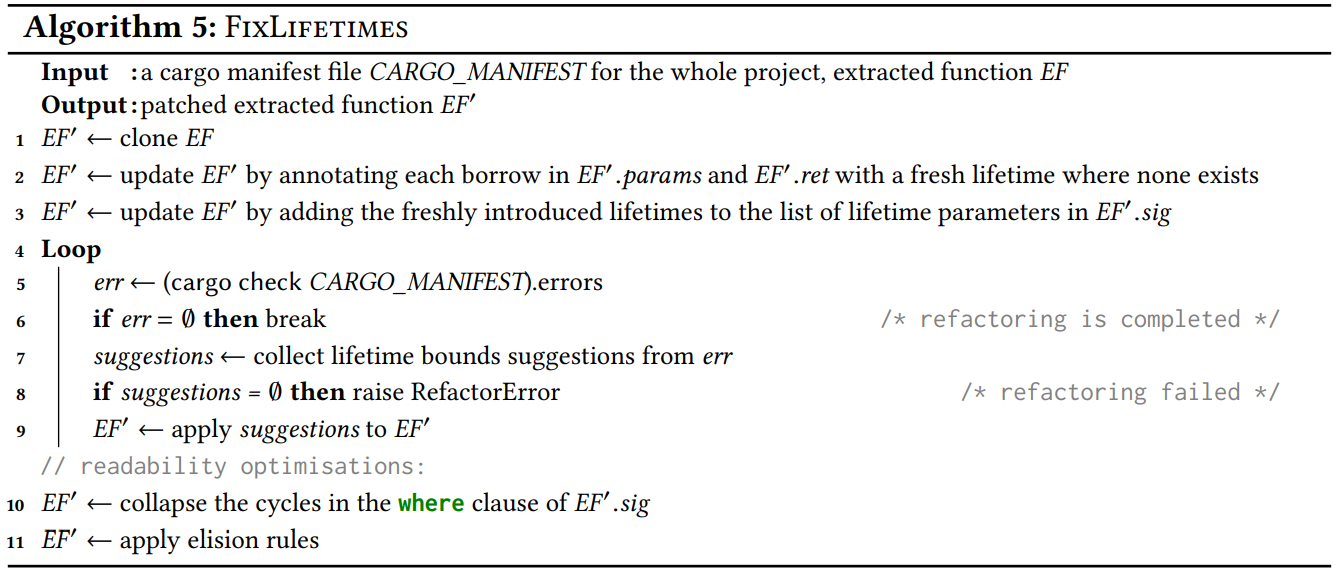
\includegraphics[width=\textwidth]{figures/algo_5.png}
    % \caption{Lifetime Repair}
    \label{fig:algo_5}
\end{figure*}

%----------------------------------------------------------------------------------------

\end{document}